\subsection{Video-Produktion}
\subsubsection{Einarbeitung in After Effects}
Zunächst einmal erfolgte eine intensive Einarbeitungsphase mit dem Programm „After Effects“. Dabei waren sehr gute Youtube Tutorials eine große Unterstützung. 
Das Resultat von dem ersten Testvideo schaut wie folgt aus: 
\begin{figure}[h]
\centering
 \subfloat[Screenshot: After Effects 1]{{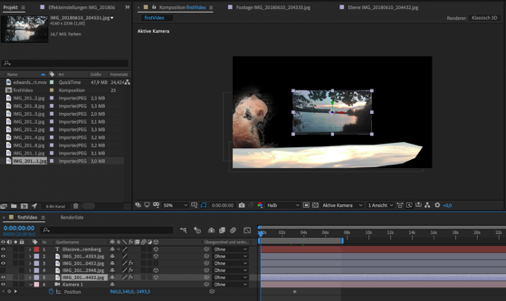
\includegraphics[width=5cm]{../img/screenshot_aftereffects_1.PNG} }}
\qquad
 \subfloat[Screenshot: After Effects 2]{{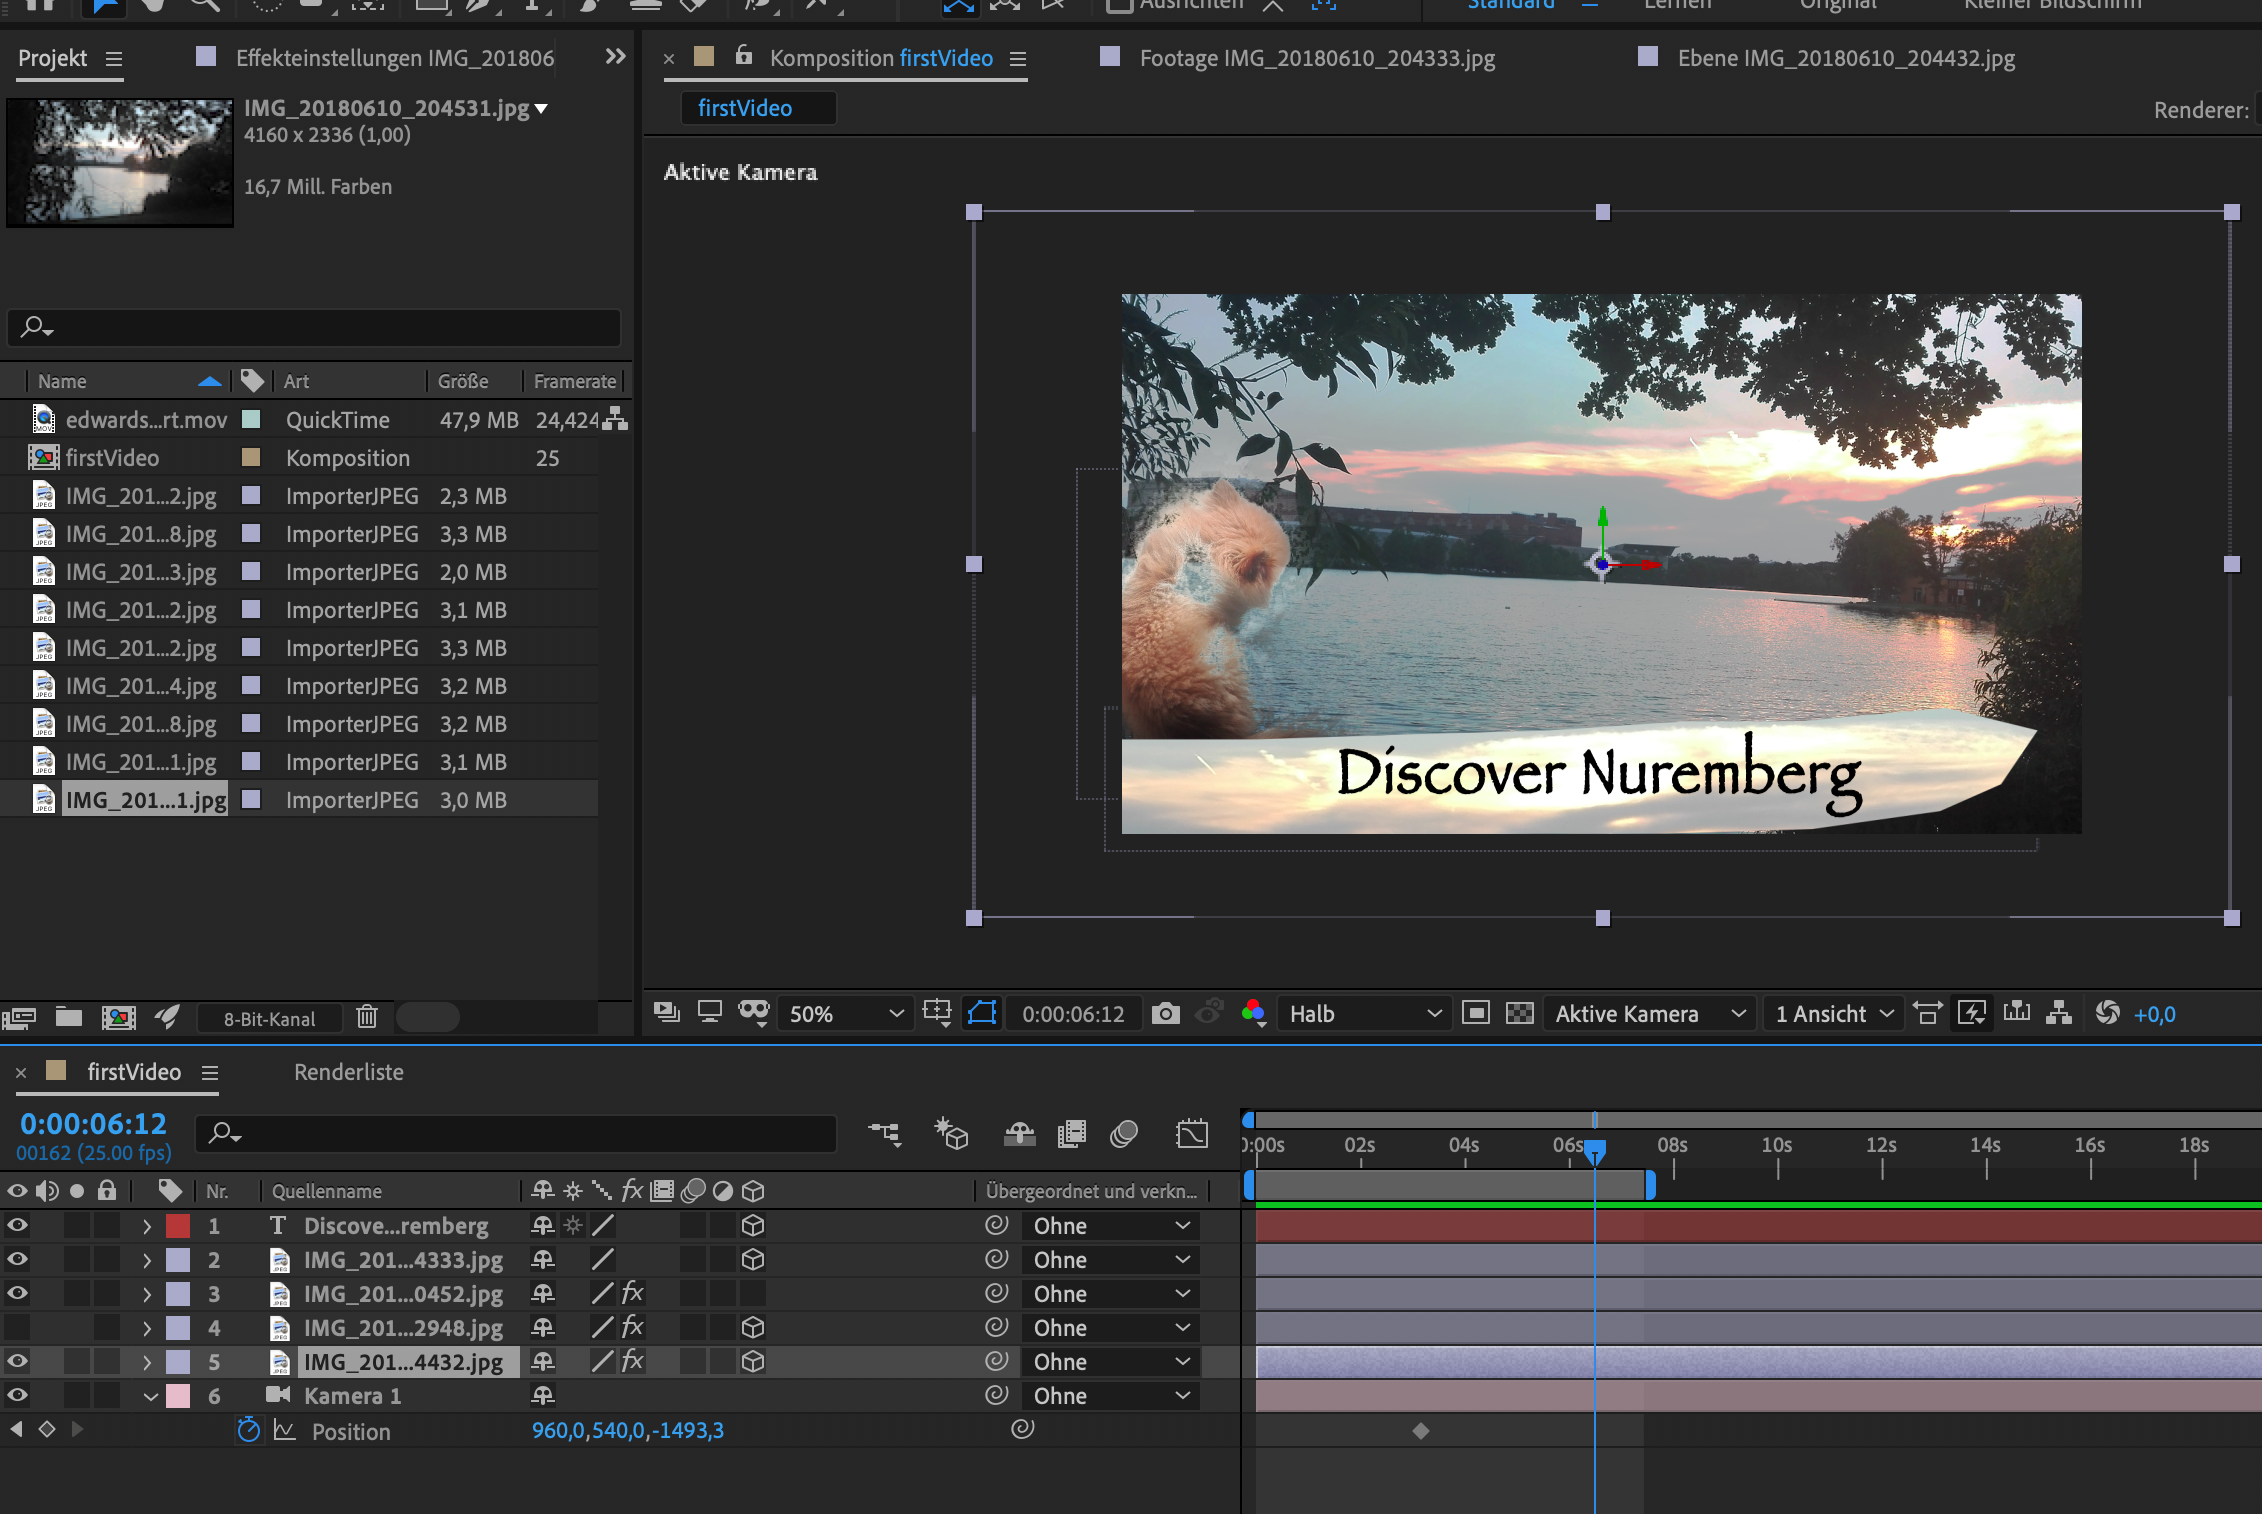
\includegraphics[width=5cm]{../img/screenshot_aftereffects_2.PNG} }}
\caption{Screenshots After Effects}%
 \label{fig:Screenshots After Effect}%
\end{figure}
Hierbei wurden Bilder freigestellt, ein Bild und der Titel animiert.  

\subsubsection{Animation des Logos}
Das Video endet, wie in vielen bekannten Videos, mit unserem Logo. Hierfür musste das Edwards Biotope Logo animiert werden. 
Zunächst einmal wurde die Grafik (links) von dem Text (rechts) separiert. Die Absicht war es, zuerst das Symbol animiert einzublenden. Im Anschluss taucht der Name „Edwards Biotope“ auf. Dieser Text wurde ebenso animiert. Zum Schluss werden beide Teile wieder zusammengefügt. Die Bildreihenfolge Abbildung \ref{fig:Screenshots Animations 1} stellt diese Logo Animation dar. 
\begin{figure}[h]
\centering
 \subfloat[Screenshot: Animation 1]{{
\includegraphics[width=2cm]{../img/logo_animation/1/screenshot_logo_1.PNG} }}
\qquad
 \subfloat[Screenshot: Animation 2]{{
\includegraphics[width=2cm]{../img/logo_animation/1/screenshot_logo_2.PNG} }}
\qquad
 \subfloat[Screenshot: Animation 3]{{
\includegraphics[width=2cm]{../img/logo_animation/1/screenshot_logo_3.PNG} }}
\qquad
 \subfloat[Screenshot: Animation 4]{{
\includegraphics[width=2cm]{../img/logo_animation/1/screenshot_logo_4.PNG} }}
\caption{Screenshots Animations 1}%
 \label{fig:Screenshots Animations 1}%
\end{figure}

Allerdings war das nicht sehr überzeugend. Daher wurde weiterhin experimentiert. So wurde das Logo mit dem Spielnamen nicht mehr separiert animiert, sondern von Anfang an zusammen. Der Bildablauf  Abbildung \ref{fig:Screenshots Animations 2} veranschaulicht diese Animation.

\begin{figure}[h]
\centering
 \subfloat[Screenshot: Animation 5]{{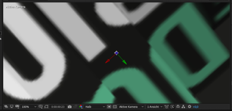
\includegraphics[width=2cm]{../img/logo_animation/2/screenshot_logo_5.PNG} }}
\qquad
 \subfloat[Screenshot: Animation 6]{{
\includegraphics[width=2cm]{../img/logo_animation/2/screenshot_logo_6.PNG} }}
\qquad
 \subfloat[Screenshot: Animation 7]{{
\includegraphics[width=2cm]{../img/logo_animation/2/screenshot_logo_7.PNG} }}
\caption{Screenshots Animations 2}%
 \label{fig:Screenshots Animations 2}%
\end{figure}

Im Anschluss wurde ein CC Light Sweep Effekt hinzugefügt und dafür gesorgt, dass das Logo kurz glänzt. Mit der Bestimmung der Richtung verläuft dieser Effekt von links oben nach rechts unten. Dieser Effekt ist auf der Abbildung \ref{fig:Screenshots Animations 3} zu sehen.

\begin{figure}[h]
\centering
 \subfloat[Screenshot: Animation 8]{{
\includegraphics[width=2cm]{../img/logo_animation/3/screenshot_logo_8.PNG} }}
\qquad
 \subfloat[Screenshot: Animation 9]{{
\includegraphics[width=2cm]{../img/logo_animation/3/screenshot_logo_9.PNG} }}
\qquad
 \subfloat[Screenshot: Animation 10]{{
\includegraphics[width=2cm]{../img/logo_animation/3/screenshot_logo_10.PNG} }}
\caption{Screenshots Animations 3}%
 \label{fig:Screenshots Animations 3}%
\end{figure}